\chapter{Summary and further work}

\label{ch:summary}

\section{Structure properties and intrinsic defects in \zirconia}

DFT calculations of non-defective \zirconia\ predicted the correct order of phase stability for the monoclinic, tetragonal and cubic phases. Calculated lattice parameters of each phase also agreed to within 2\% of experimental values. Calculated band gaps of each phase were underestimated by approximately 2 eV, which is typical when modelling using GGA-DFT. A Hubbard +U study revealed that the calculated band gaps could be increased by up to 1 eV, but that the symmetry of the supercells would be distorted in the process.

Helmholtz free energy calculations at temperatures ranging from 0 to 2500 K showed that the lowest energy phase changes from monoclinic to tetragonal, but not from tetragonal to cubic. Furthermore, the predicted transition temperature of the monoclinic-tetragonal phase change is underestimated by almost 1100 K. This is attributed to lack of thermal expansion in the constant-volume harmonic model but could also be a consequence of the kinetic barrier of the phase transformation.

Elastic constants were calculated and reported for each phase. The cubic phase was predicted to have the highest stiffness, followed by monoclinic and then tetragonal. The elastic constants were used to calculate the bulk modulus of each phase, and it was shown that the monoclinic and tetragonal bulk moduli agreed with experimental values to within 5\%. The calculated bulk modulus in the cubic phase could not be compared to an experimental value in pure \zirconia , but was 15\% larger than that of YSZ.

Formation energy calculations showed that Zr vacancies in all three phases are fully-charged (\ch{V_{Zr}^{''''}}) over most Fermi levels, while O vacancies change from \ch{V_{O}^{**}} at low Fermi levels to \ch{V_{O}^{x}} when the Fermi level is larger than 3 eV. The defect cluster with the lowest formation energy per defect was the fully-charged Schottky, followed by O Frenkel defects and then Zr Frenkel defects. This can be partly attributed to defect sizes, with Schottky defects predicted to have the smallest defect volumes in all phases, again followed by O Frenkel defects and then Zr Frenkel defects.

Brouwer diagrams were constructed for each phase, and showed that the defect equilibria are dominated by \ch{V_{Zr}^{''''}}, \ch{V_{O}^{**}}, \ch{h^{*}} and \ch{e^{'}} defects. Interstitial defects appear only at very low concentrations relative to these defects. This suggests that Schottky defects will be the main cluster defect near stoichiometry. At high $p_{O_{2}}$, \ch{V_{Zr}^{''''}} is charge-compensated by \ch{h^{*}} defects, while at low $p_{O_{2}}$, \ch{V_{O}^{**}} is charge-compensated by \ch{e^{'}} defects.

Cubic \zirconia\ supercells sometimes exhibited a loss of symmetry when performing defect energy minimisations. This behaviour and anomalous results from other calculations led to the conclusion that the cubic phase might not be modelled accurately with present DFT methods. Work by Burr \emph{et al.} \cite{burr2017importance} supports this result. In addition, the high temperatures required to stabilise the cubic phase limit the ability to examine defect equilibria due to the high intrinsic defect concentrations. Cubic phase Brouwer diagrams were therefore not constructed in subsequent extrinsic defect studies.

\section{Iodine doping and oxygen competition}

Iodine point defects were studied in the three phases to investigate defect energies and these were used to construct Brouwer diagrams in the monoclinic and tetragonal phases. It was found that in monoclinic \zirconia , iodine has lower incorporation energies onto both Zr and O sites than in the tetragonal phase. In all phases, \ch{I_{O}} defects exhibit the smallest incorporation energies, followed by \ch{I_{Zr}} and then \ch{I_{i}}. 

Four unique interstitial sites for iodine were found in the monoclinic phase, and two in the tetragonal and cubic phases. It was found that the lowest energy interstitial sites changed in the tetragonal and cubic phases depending on the Fermi level, whereas only one site was favourable in the monoclinic phase. Iodine interstitial defects will only exist as \ch{I_{i}^{*}} at low Fermi levels or \ch{I_{i}^{'}} at high Fermi levels, whereas \ch{I_{i}^{x}} defects will have a higher formation energy regardless of the Fermi level. At the O site, iodine will form \ch{I_{O}^{*}} and to a lesser extent, \ch{I_{O}^{***}} defects. At the Zr site, iodine will form \ch{I_{Zr}^{'''}} defects. 

Brouwer diagrams showed that there is competition between iodine and oxygen for anion sites in \zirconia , and that this competition is dependent on both phase and oxygen pressure. It was found that higher oxygen pressures will reduce the equilibrium concentration of \ch{I_{O}} and \ch{I_{i}} defects in both phases, but with a more significant effect in the tetragonal phase. A combination of high oxygen pressure and tetragonal phase led to oxygen out-competing iodine for anion sites. This will reduce diffusion rates of iodine in the oxide layer.

% iodine interstitial defects are predicted to be mostly \ch{I_{i}^{*}}, and will be observed in higher concentrations in monoclinic \zirconia . This is likely due to the larger size of the interstitial sites and therefore better accommodation of the large iodine atom.

\section{Decay chain elements in \zirconia}

I nuclei produced during nuclear fission are unstable and will therefore be part of a decay chain. Decay of Te precursors are the major source of I. Furthermore, Xe and Cs are predicted to be present in significant concentrations based on decay rates and fission yields. Decay rates of Te and I isotopes were also found to be commensurate with the time taken for PCI failures to occur following a power ramp, hinting that these phenomena may be related. From the iodine study, tetragonal phase \zirconia\ was predicted to provide a greater barrier effect against iodine. Thus, defect equilibria and defect volumes of decay chain elements Te to Cs were investigated in tetragonal \zirconia . 

Brouwer diagrams predicted low concentrations of interstitial defects relative to O and Zr substitutional defects. At the O site, the defect evolution is predicted to be \ch{Te_{O}^{**}} $\rightarrow$ \ch{I_{O}^{*}} $\rightarrow$ \ch{Xe_{O}^{**}} $\rightarrow$ \ch{Cs_{O}^{**}} while at the Zr site, the Brouwer diagrams predict \ch{Te_{Zr}^{'''}} $\rightarrow$ \ch{I_{Zr}^{'''}} $\rightarrow$ \ch{Xe_{Zr}^{''''}} $\rightarrow$ \ch{Cs_{Zr}^{'''}}.

As Te decays towards Xe, the defects produced have progressively larger volumes. All substitutional defects have positive volumes ranging from +21 to +46 \r{A}$^{3}$ relative to the non-defective crystal, with the largest major defect being \ch{I_{O}^{*}} (46.94 \r{A}$^{3}$). All O substitutional defects were found to be larger than those on the Zr site. The stresses generated by defects on a constrained supercell were also calculated and shown to follow the same trends as the defect volumes.

Stresses imposed by implanted fission products and their decay chain elements will promote the formation of new surfaces. During a power ramp, the rate of fission product implantation within the oxide will increase. The largest stresses will occur in the hours following the ramp when I concentrations reach a maximum level. Stresses will begin to fall as more I nuclei decay into Xe and Cs, which have smaller defect volumes. This mechanism is proposed as a contributing factor to PCI failures, as larger ramps are more likely to lead to failure and the rate of new crack formation may exceed the rate at which a passivating oxide is developed.

\section{Further work}

\subsection{Temperature effects in intrinsic defect simulations}

ZrO$_{2}$ crystal structures are sensitive to changes in interatomic spacing, sometimes causing a loss of supercell symmetry when defects are modelled. There is a need to accurately represent anisotropic effects such as thermal expansion in the different phases over a broad temperature range. This can be achieved by developing potentials and conducting classical or quantum MD simulations to test their performance through comparison to experimental data. Quantum MD simulations, however, are very computationally expensive. A good starting point is to perform phonon calculations of the different ZrO$_{2}$ phases in conjunction with the quasi-harmonic method. This is an extension to the method outlined in § \ref{helmholtz_method} which can be used to find the ground state lattice positions (and therefore interatomic spacings) at different temperatures. These values are used to determine thermal expansion coefficients of ZrO$_{2}$ along each lattice vector. Potentials can then be developed with these thermal expansion coefficients, which will be able to reproduce the anisotropic effects in different phases.

\subsection{Fission product empirical potential}

In order to study the interaction of fission products with larger features in the cladding microstructure, such as dislocations and grain boundaries, it is necessary to develop empirical potentials for use in molecular dynamics simulations. Grain boundary transport is of particular interest, but this would require something on the order of 10$^{4}$ atoms to represent a system large enough to develop a reasonable degree of accuracy. This cannot currently be achieved using DFT due to the significant amount of computing resources required to run such a simulation. 

The development of an iodine and xenon potential with \zirconia\ should be prioritised in order to run simulations to determine the migration of iodine within \zirconia, followed by the behaviour of xenon at sites occupied by iodine.

\subsection{Zr/ZrO/\zirconia\ interface study}

The inner oxide is not a homogeneous structure, as described in Chapter \ref{ch:crystallography}. Figure \ref{fig:zro_interface} shows the existence of a ZrO phase up to 200 nm thick at the interface between \zirconia\ and Zr metal. The presence of ZrO and even oxygen-saturated Zr metal will have an effect on the thermodynamic equilibria of different fission products. An interface study can be conducted using DFT, to determine stresses at the interfaces of Zr and ZrO, and ZrO and \zirconia . Studying the aggregate effect of these interfaces on fission product behaviour may require larger molecular dynamics simulations. 

The crystal structure of the ZrO phase has been studied using both simulation and high-resolution electron microscopy, with two likely crystal structures being proposed \cite{Nicholls2015}. Further atomistic studies must be conducted to determine the stability of each crystal structure of ZrO when constrained by \zirconia\ and oxygen-saturated Zr metal interfaces (i.e. can we determine if stress stabilises the ZrO layer?).

\begin{figure}[ht] % ZrO interface
    \centering
    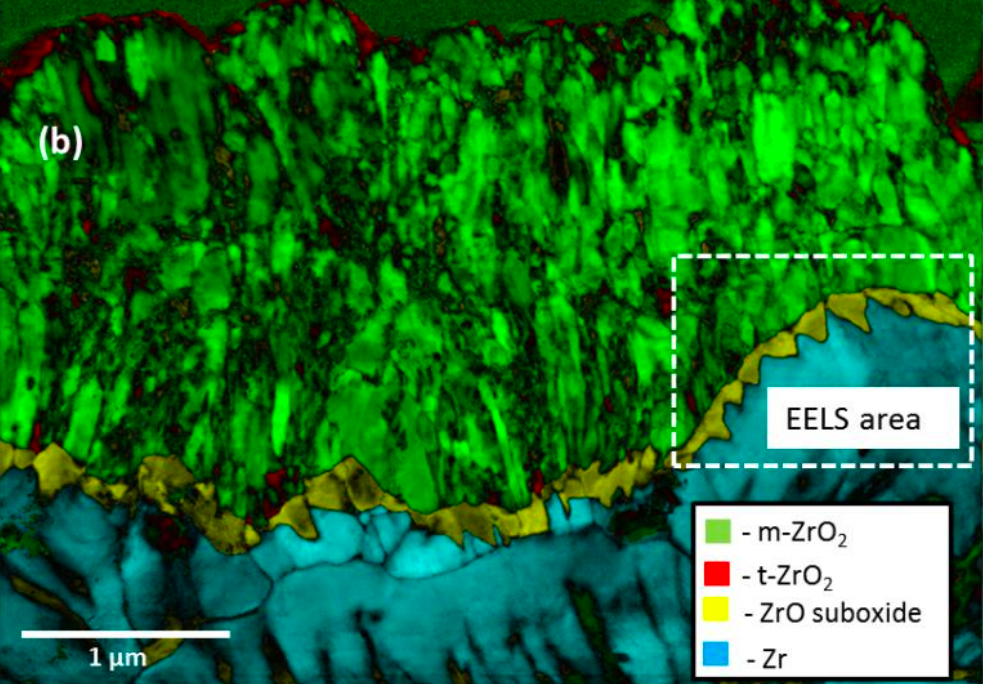
\includegraphics[height=9cm]{images/zro_interface.png}
    \caption[STEM image of a Zr-1.0\%Nb sample oxidised in simulated PWR water at 360 \textdegree C for 120 days.]{STEM image of a Zr-1.0\%Nb sample oxidised in simulated PWR water at 360 \textdegree C for 120 days. Taken from \cite{inproceedings}.}
    \label{fig:zro_interface}
\end{figure}

\subsubsection{Bromine}

Bromine is another halogen atom produced from fission, although in smaller quantities than iodine. Since bromine has similar chemical behaviour to iodine, though it is somewhat smaller (I$^{-}$ radius = 2.20 \r{A}, Br$^{-}$ radius = 1.96 \r{A} \cite{Shannon1976}), it would be of interest to conduct a defect study with bromine in \zirconia\ similar to that in Chapter \ref{ch:results2}. Iodine produced defects which were in either the +1 or -1 oxidation states (e.g. \ch{I_{Zr}^{'''}} and \ch{I_{O}^{*}}). This would help determine if Br defects also exhibit this behaviour, or if the 0 oxidation state demonstrates greater stability at certain sites. Furthermore, the pathway to Br isotopes will be different to I in terms of decay rates and this must also be considered.

\subsection{Defect volumes}

Defect volumes are useful quantities for comparing different defects and explaining their behaviour, however, the calculation of defect volumes for charged defects in DFT models is a contentious topic. While defect volumes of charged point defects are often reported in the literature, reported values are often unphysically large \cite{Bruneval2015}. For this reason, the charged defect volumes reported in this thesis used the volume of an equivalently charged non-defective supercell as the reference volume. This method has been shown to yield more reasonable defect volumes for charged defects \cite{goyal2017conundrum}, but this is still only a rudimentary correction. 

One method for obtaining more accurate defect volumes is to use larger supercells (to reduce finite size effects and self-interaction errors across the periodic boundary). Another possibility is using hybrid-AE functionals which reproduce a more accurate electronic band structure, thereby reducing energy errors and improving the accuracy of interatomic forces when adding or removing electrons in a defective system with non-zero charge \cite{Brothers2008}.
% \cite{He2006} Jellium

\subsection{Experimental work}

\subsubsection{Tetragonal phase stabilisation}

A key finding in this thesis is that tetragonal phase \zirconia\ (as opposed to monoclinic) provides the barrier effect against corrosive fission products. It would therefore be useful to conduct experiments on claddings designed to maximise the content of tetragonal phase \zirconia\ in the internal oxide layer. While this can be achieved with a tetragonal stabilising dopant (e.g. scandium or yttrium), this will increase the concentration of oxygen vacancies which may lead to reduced corrosion performance. 

Another method to increase the proportion of tetragonal phase in the oxide layer is to reduce the Zr grain size. This is an attractive option because the chemical composition of the cladding will be unchanged, and the increased strength does not come at the cost of ductility. The very small grain sizes required (nanoscale) will, however, negatively impact the creep resistance of the cladding, so if this is not a realistic modification for the entire clad, it may be better to refine only the Zr liner grain size. 

\subsubsection{Oxygen environment control}

A key result in Chapter \ref{ch:results2} was that at a high enough $p_{O_{2}}$ above stoichiometry, the concentration of \ch{I_{O}} and \ch{I_{i}} defects began to fall significantly, indicating competition between oxygen and iodine for anion sites in tetragonal \zirconia . Increasing the $p_{O_{2}}$ in fuel pins may therefore impede the bulk diffusion of iodine through the oxide layer, slowing the corrosion process. In-pile irradiation tests (e.g. power ramps, high burn-up behaviour) to examine the effect of increasing the oxygen content in fuel pins would provide useful data on PCI performance. Presently, fuel pins are filled with helium because it is an inert gas, it does not affect the neutronics within the core and has a high thermal conductivity (compared to other gases). One option for varying oxygen content in a fuel pin is to use a fill gas which is a mixture of helium and oxygen. Although oxygen (most of which is \ch{O^{16}_{8}}) is not inert and has a lower thermal conductivity than helium, it is highly resistant to neutron activation due to a combination of very low thermal neutron absorption cross-section and three stable isotopes (i.e. three consecutive neutron captures are required to produce an unstable \ch{O^{19}_{8}} nucleus). Adding oxygen to the fill gas is also a much simpler (and therefore cheaper) method of increasing oxygen content compared to changing the stoichiometry of the fuel.

